\subsection*{Основное состояние БКШ}


Рассмотрим основное состояние <<спаренных>> электронов в терминах вторичного квантования:
\begin{equation}
	\ket{\psi_G} = \prod_{\vc{k}} \left(
		u_{\vc{k}} + v_{\vc{k}} \hat{c}\D_{\vc{k} \up} \hat{c}\D_{-\vc{k}\down}
	\right) \ket{\psi_0},
	\label{GroundBCS}
\end{equation}
где $\psi_0$ -- вакуумное состояние. 

Количество спаренных частиц может быть найдено через оператор полного числа частиц
\begin{equation*}
	\hat{N} = \sum_{\vc{k}}  \hat{c}\D_{\vc{k} \up} \hat{c}_{\vc{k} \up} + \hat{c}\D_{\vc{k} \down} \hat{c}_{\vc{k} \down}.
\end{equation*}
Прямым вычислением, находим
\begin{equation*}
	\langle N\rangle = \bk{\psi_G}[\hat{N}]{\psi_G} = 2 \langle \textstyle\sum_{\vc{k}} \hat{N}_{\vc{k} \up} \rangle 
	= 2 \sum_{\vc{k}} \bra{\psi_0}
	 \left(
		u_\vc{k} + v_{\vc{k}}^* \hat{c}_{-\vc{k}\down} \hat{c}_{\vc{k} \up}
	\right)
	\hat{c}_{\vc{k} \up}\D \hat{c}_{\vc{k} \up} 
	(
		u_k + v_k \hat{c}\D_{\vc{k} \up} \hat{c}_{-\vc{k}\down}\D
	) \ket{\psi_0} = 2 \sum_{\vc{k}} |v_{\vc{k}}|^2,
\end{equation*}
как и ожидалось. 





\subsection*{Вариационный метод}


Гамильтониан системы почти идеального ферми-газа запишется \cite{ll9}
\begin{equation*}
	\hat{H} = \sum_{\vc{k}} \varepsilon_{\vc{k}} \left(
		\hat{c}\D_{\vc{k} \up} \hat{c}_{\vc{k} \up} + \hat{c}\D_{\vc{k} \down} \hat{c}_{\vc{k} \down}
	\right) + \sum_{\vc{k},\, \vc{k}'} V_{\vc{k} \vc{k}'} c\D_{\vc{k} \up} \hat{c}\D_{-\vc{k}' \down} \hat{c}_{-\vc{k}' \down} \hat{c}_{\vc{k}' \up}.
\end{equation*}
Чтобы явно не учитывать постоянство числа частиц в системе \cite{ll9} в качестве нового гамильтониана вводится разность $\hat{H} \to \hat{H} - \mu \hat{N}$. Коэффициенты в \eqref{GroundBCS} найдём минимизируя 
\begin{equation*}
	\mathbb{E} \overset{\mathrm{def}}{=}  \bk{\psi_G}[\hat{H} - \mu \hat{N}]{\psi_G},
	\hspace{10 mm} 
	\delta \mathbb{E} = 0.
\end{equation*}
Введем также обозначение
\begin{equation*}
	\xi_{\vc{k}} \overset{\mathrm{def}}{=} \varepsilon_{\vc{k}} - \mu.
\end{equation*}
Аналогично вычислению $\langle N\rangle$, находим 
\begin{equation*}
	\mathbb{E} = 2 \sum_{\vc{k}} \xi_{\vc{k}} |v_{\vc{k}}|^2 + \sum_{\vc{k} \vc{k}'} V_{\vc{k}' \vc{k}} u_{\vc{k}'} v_{\vc{k}'}^* u_{\vc{k}}^* v_{\vc{k}}.
\end{equation*}
Считая $u_{\vc{k}},\, v_{\vc{k}} \in \mathbb{R}$, сделаем подстановку
\begin{equation*}
	u_k = \sin \theta_k,
	\hspace{10 mm} 
	v_k = \cos \theta_k.
\end{equation*}
Тогда минимизируемая величина запишется в виде
\begin{equation*}
	E = \sum_{\vc{k}} \xi_{\vc{k}} \left(1 + \cos 2 \theta_{\vc{k}}\right) + 
	\frac{1}{4} \sum_{\vc{k}\, \vc{k}'} V_{\vc{k} \vc{k}'}\sin(2 \theta_k) \sin(2 \theta_{\vc{k}'}).
\end{equation*}
Считая $\partial_{\theta_{\vc{k}}} \mathbb{E} =0$,  находим
\begin{equation*}
	- 2 \xi_{\vc{k}} \sin\left(2 \theta_{\vc{k}}\right) + \sum_{\vc{k}'} V_{\vc{k} \vc{k}'} \cos\left(2 \theta_{\vc{k}}\right) \sin(2 \theta_{\vc{k}'}),
	\hspace{0.5cm} \Rightarrow \hspace{0.5cm}
	\tg \theta_{\vc{k}} = \frac{1}{2 \xi_{\vc{k}}} \sum_{\vc{k}\, \vc{k}'} V_{\vc{k} \vc{k}'} \sin\left(2 \theta_{\vc{k}'}\right).
\end{equation*}
Теперь можем ввести две величины:
\begin{equation*}
	\Delta_{\vc{k}} \overset{\mathrm{def}}{=}  - \sum_{\vc{k}'} V_{\vc{k} \vc{k}'} u_{\vc{k}'} v_{\vc{k}'} = - \frac{1}{2} \sum_{\vc{k}'} V_{\vc{k} \vc{k}'} \sin\left(2 \theta_{\vc{k}'}\right),
	\hspace{10 mm} 
	E_{\vc{k}} = \sqrt{\Delta_{\vc{k}}^2 + \xi_{\vc{k}}^2}.
\end{equation*}
Тогда явно находим
\begin{equation}
	\sin(2 \theta_k) = 2 u_{\vc{k}} v_{\vc{k}} = \frac{\Delta_{\vc{k}}}{E_{\vc{k}}},
	\hspace{5 mm} 
	\cos(2 \theta_{\vc{k}}) = v_{\vc{k}}^2 - u_{\vc{k}}^2 = - \frac{\xi_{\vc{k}}}{E_{\vc{k}}}.
	\label{uvEqs}
\end{equation}
Тогда уравнение на ширину запрещенной зоны запишется в виде
\begin{equation}
	\Delta_{\vc{k}} = - \frac{1}{2} \sum_{\vc{k}'} \frac{\Delta_{\vc{k}'}}{E_{\vc{k}'}} V_{\vc{k} \vc{k}'} = - \frac{1}{2} \sum_{\vc{k}'}  V_{\vc{k} \vc{k}'} \frac{\Delta_{\vc{k}'}}{\sqrt{\Delta_{\vc{k}'}^2 + \xi_{\vc{k}'}^2}}.
	\label{DeltaEq}
\end{equation}





\subsection*{Подстановка Купера}

Сначала Купером \cite{cooper}, а затем в рамках модели БКШ было предложено использовать потенциал, вида
\begin{equation*}
	V_{\vc{k} \vc{k}'} = \left\{\begin{aligned}
	    &-V, &|\xi_{\vc{k}}|, |\xi_{\vc{k}'}| \leq \Theta_{D} \\
	    &0, &\text{иначе}
	\end{aligned}\right.
\end{equation*}
где $\Theta_{D}$ -- температура Дебая, размерности энергии. 

Тогда \eqref{DeltaEq} запишется в виде
\begin{equation*}
	1 = \frac{V}{2} \sum_{\vc{k}'} \frac{1}{E_{\vc{k}'}} = N(0) V \int_{0}^{\Theta_D} \frac{1}{\sqrt{\Delta^2  + \xi^2}} \d \xi = N(0) V \arcsh\left(\frac{\Theta_D}{\Delta}\right),
	\hspace{0.5cm} \Rightarrow \hspace{0.5cm}	\Delta \approx 2 \Theta_D e^{- \frac{1}{N(0) V}},
\end{equation*}
где сделано приближение $D(E) \approx D(E)|_{E=E_F} = N(0)$.



Уравнения \eqref{uvEqs} позволяют в явном виде найти
\begin{equation*}
	\left.\begin{aligned}
	    u_{\vc{k}}^2 \\
	    v_{\vc{k}}^2
	\end{aligned}\right\}
	= \frac{1}{2} \left(1 \pm \frac{\xi_{\vc{k}}}{E_{\vc{k}}}\right) = \frac{1}{2}\left(
		1 \pm \frac{\xi_{\vc{k}}}{\sqrt{\Delta^2 + \xi_{\vc{k}}^2}}
	\right),
\end{equation*}
явная зависимость $|v_{\vc{k}}|^2(\xi_{\vc{k}})$ приведена на рис. \ref{fig:1}.	



\begin{figure}[h]
    \centering
    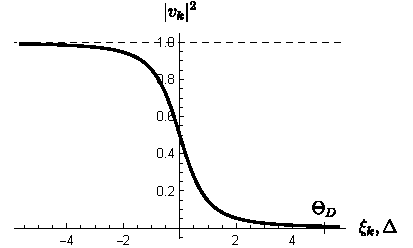
\includegraphics[width=0.4\textwidth]{plot_1.pdf}
    \hspace{10 mm} 
    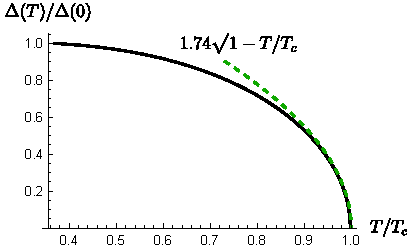
\includegraphics[width=0.4\textwidth]{plot_2.pdf}
    \caption{Зависимость $|v_{\vc{k}}|^2(\xi_{\vc{k}})$ при $T=0$ и $N(0) V = 0.43$, зависимость $\Delta(T)$}
    \label{fig:1}
\end{figure}


